% How The Yardstick decides, Vagrancy (data/pilots.json, "yardstick": a search pilot,
% horizon_ticks 20, reaction_ticks 10, branches 11, period 5). It has no rules: every
% decision is one look-ahead search, drawn here as a search tree.
% Standalone: compiles on its own in Overleaf with pdflatex.
\documentclass[tikz,border=4pt]{standalone}
\usetikzlibrary{arrows.meta,shapes.geometric,positioning,calc}

% --- Colors: the deck's palette --------------------------------------------
\definecolor{paper}{HTML}{FDFDFC}   % node fill
\definecolor{ink}{HTML}{1B2430}     % text and edges
\definecolor{muted}{HTML}{6B7680}   % notes
\definecolor{cond}{HTML}{2F4BA0}    % the world it reads
\definecolor{act}{HTML}{2A6B4A}     % key combinations and the chosen move
\definecolor{score}{HTML}{8B2E2E}   % scoring

% --- Settings: the yardstick's entry in data/pilots.json ----------------------
\newcommand{\Reaction}{10}     % reaction_ticks: how old the world it decides on is
\newcommand{\ReactionMs}{167}  % the same in ms, ceil(10 x 1000 / 60)
\newcommand{\Horizon}{20}      % horizon_ticks: how far each candidate is simulated
\newcommand{\HorizonMs}{334}   % the same in ms, ceil(20 x 1000 / 60)
\newcommand{\Period}{5}        % period: ticks it holds a choice before searching again

% --- Layout, in centimetres --------------------------------------------------
\newcommand{\Cell}{0.72}       % width of one tick in the history strip
\newcommand{\StripY}{1.6}      % height of the history strip
\newcommand{\RowGap}{1.0}      % vertical distance between candidates
\newcommand{\TopRow}{-0.4}     % height of the first candidate
\newcommand{\RootX}{2.9}       % the copied world
\newcommand{\CandX}{8.4}       % the key combinations
\newcommand{\FutureX}{13.9}    % the simulated futures
\newcommand{\PickX}{18.2}      % the choice
\newcommand{\ScoreX}{21.2}     % left edge of the score panel

\begin{document}
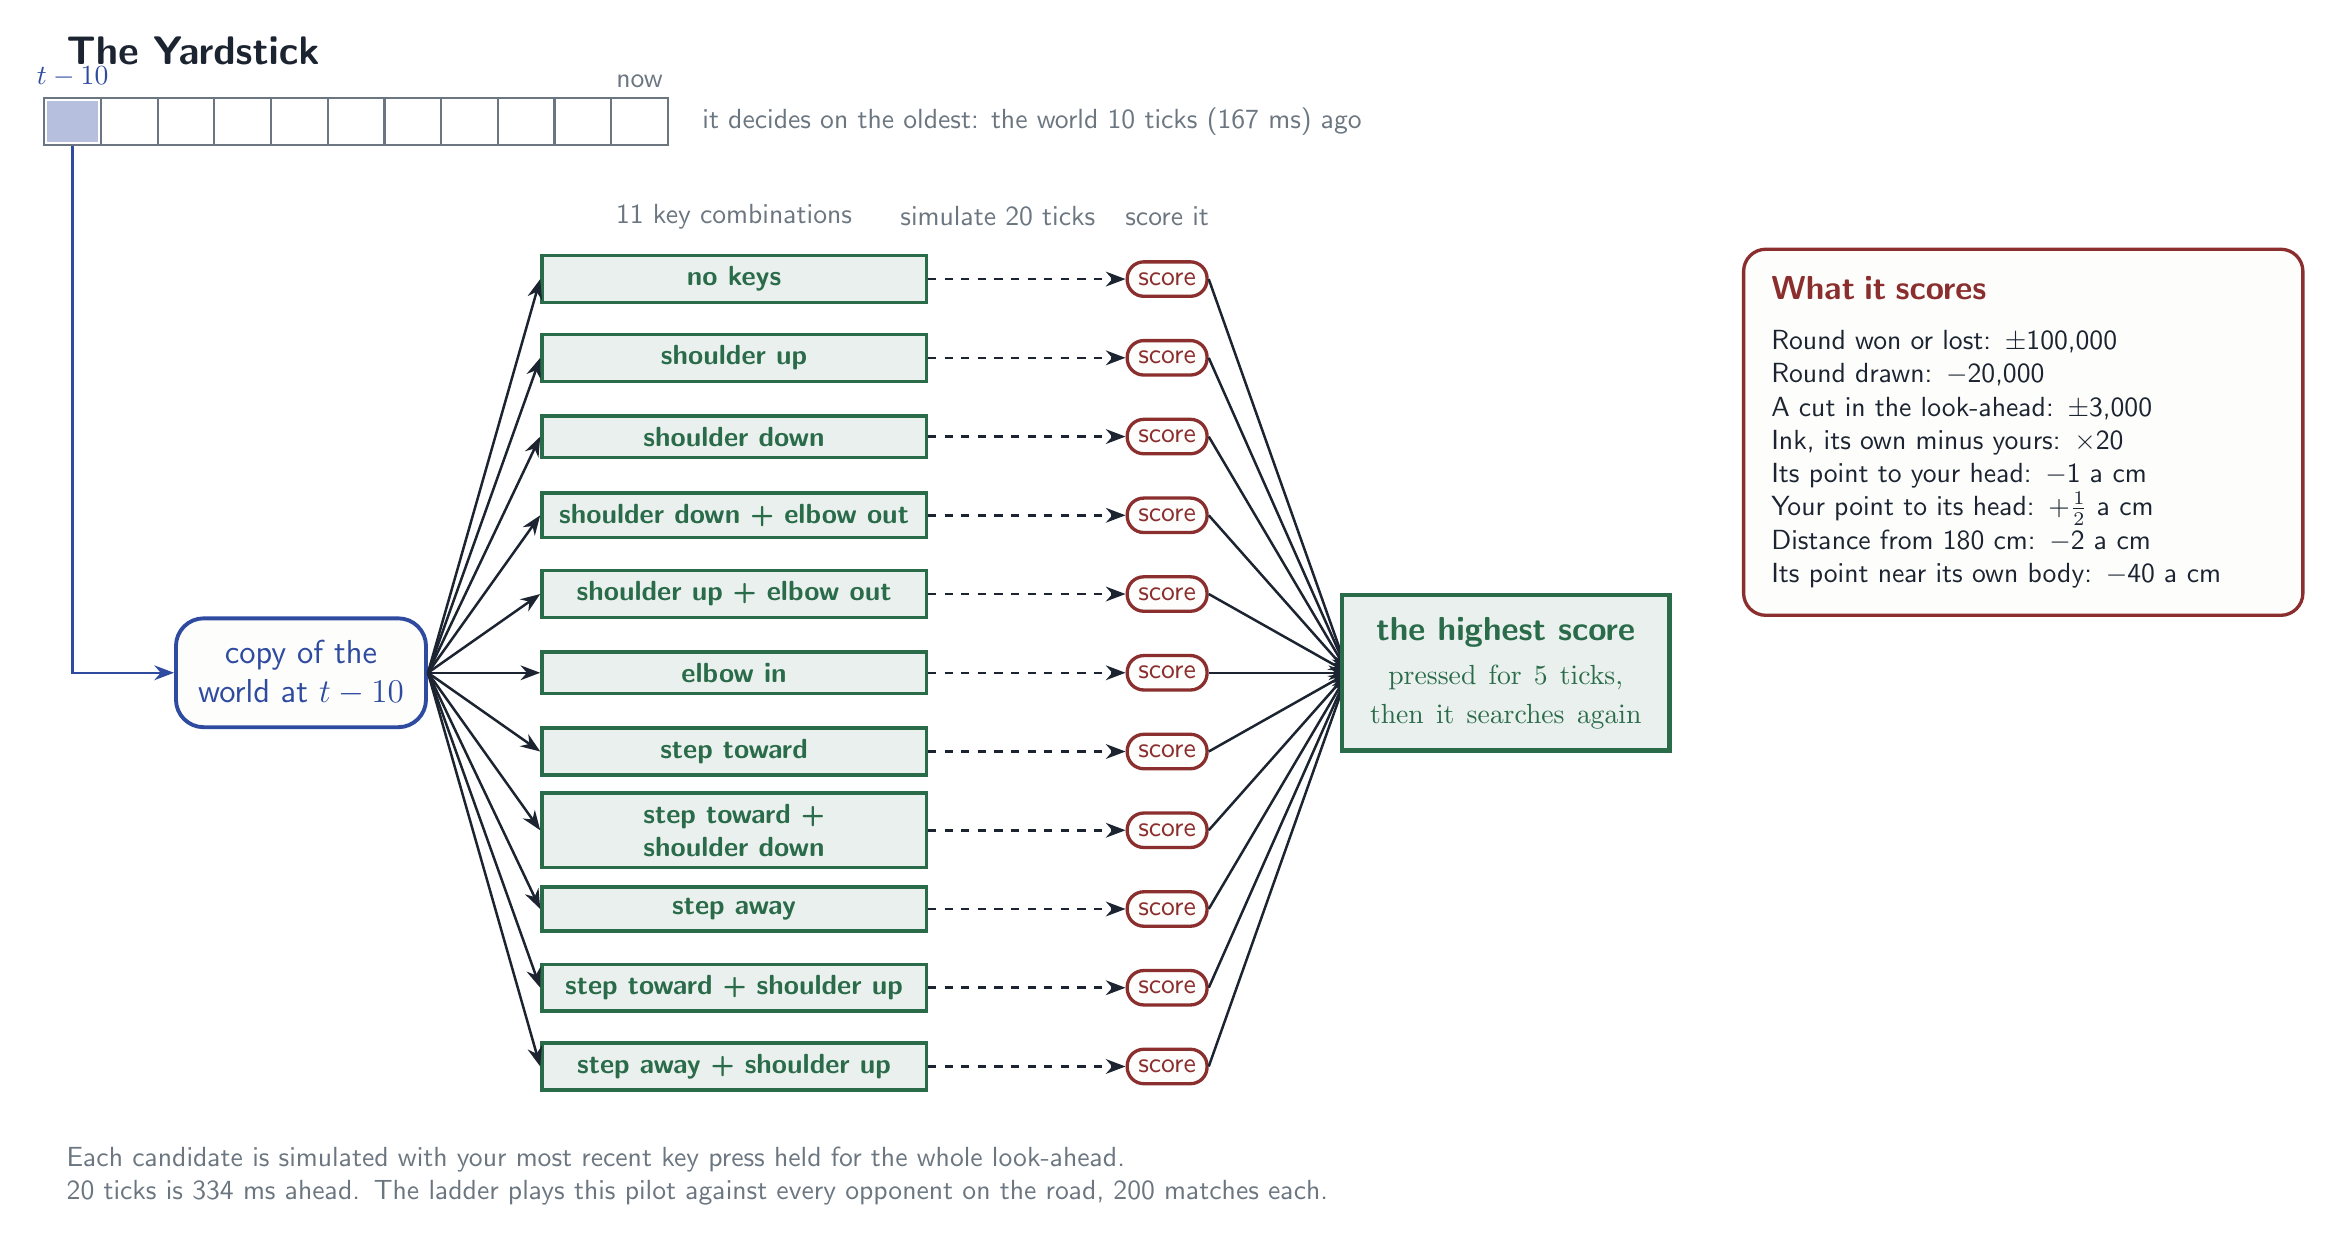
\begin{tikzpicture}[
    font=\sffamily\large, ink,
    edge/.style={-{Stealth[length=2.5mm]}, line width=0.9pt, draw=ink},
    tick/.style={draw=muted, line width=0.8pt, minimum width=\Cell cm, minimum height=0.6cm, inner sep=0pt},
    world/.style={draw=cond, line width=1.4pt, rounded corners=10pt, fill=paper, text=cond, align=center, inner sep=8pt},
    keys/.style={draw=act, line width=1.2pt, fill=act!10, text=act, text width=4.6cm, align=center, inner sep=4pt, font=\sffamily\normalsize\bfseries},
    future/.style={draw=score, line width=1.2pt, rounded corners=6pt, fill=paper, text=score, inner sep=4pt, font=\sffamily\normalsize},
    pick/.style={draw=act, line width=1.6pt, fill=act!10, text=act, text width=3.6cm, align=center, inner sep=8pt, font=\sffamily\large\bfseries},
  ]

\node[font=\sffamily\bfseries\Large, anchor=south west] at (-0.2, \StripY+0.6) {The Yardstick};

% --- The history strip: the worlds it remembers ------------------------------
\foreach \k in {0,...,\Reaction} {
  \node[tick] (h\k) at (\k*\Cell, \StripY) {};
}
\fill[cond!35] ($(h0.south west)+(0.05,0.05)$) rectangle ($(h0.north east)-(0.05,0.05)$);
\node[anchor=south, font=\sffamily\normalsize, text=cond] at (h0.north) {$t-\Reaction$};
\node[anchor=south, font=\sffamily\normalsize, text=muted] at (h\Reaction.north) {now};
\node[anchor=west, font=\sffamily\normalsize, text=muted, align=left] at ($(h\Reaction.east)+(0.3,0)$)
  {it decides on the oldest: the world \Reaction{} ticks (\ReactionMs{} ms) ago};

% --- The copied world ----------------------------------------------------------
\pgfmathsetmacro{\MidY}{\TopRow - 5*\RowGap}
\node[world] (root) at (\RootX, \MidY) {copy of the\\world at $t-\Reaction$};
\draw[edge, draw=cond] (h0.south) |- (root.west);

% --- Eleven key combinations, each simulated \Horizon ticks ahead and scored -----
\node[font=\sffamily\normalsize, text=muted] at (\CandX, \TopRow+0.8) {11 key combinations};
\node[font=\sffamily\normalsize, text=muted] at ({(\CandX+\FutureX)/2+0.6}, \TopRow+0.8) {simulate \Horizon{} ticks};
\node[font=\sffamily\normalsize, text=muted] at (\FutureX, \TopRow+0.8) {score it};
\foreach \i/\k in {0/{no keys}, 1/{shoulder up}, 2/{shoulder down}, 3/{shoulder down + elbow out},
                   4/{shoulder up + elbow out}, 5/{elbow in}, 6/{step toward}, 7/{step toward + shoulder down},
                   8/{step away}, 9/{step toward + shoulder up}, 10/{step away + shoulder up}} {
  \pgfmathsetmacro{\y}{\TopRow - \i*\RowGap}
  \node[keys] (c\i) at (\CandX, \y) {\k};
  \node[future] (f\i) at (\FutureX, \y) {score};
  \draw[edge] (root.east) -- (c\i.west);
  \draw[edge, dashed] (c\i.east) -- (f\i.west);
  \draw[edge] (f\i.east) -- (\PickX-2.0, \MidY);
}

% --- The choice ------------------------------------------------------------------
\node[pick] (pick) at (\PickX, \MidY) {the highest score\\[2pt]{\normalfont\normalsize pressed for \Period{} ticks, then it searches again}};

% --- The score panel -------------------------------------------------------------
\node[anchor=north west, draw=score, line width=1.2pt, rounded corners=8pt, fill=paper, text width=6.4cm, inner sep=10pt, font=\sffamily\normalsize, align=left]
  at (\ScoreX, \TopRow+0.4) {\textcolor{score}{\bfseries\large What it scores}\\[6pt]
  Round won or lost: $\pm$100,000\\
  Round drawn: $-$20,000\\
  A cut in the look-ahead: $\pm$3,000\\
  Ink, its own minus yours: $\times$20\\
  Its point to your head: $-$1 a cm\\
  Your point to its head: $+\frac{1}{2}$ a cm\\
  Distance from 180 cm: $-$2 a cm\\
  Its point near its own body: $-$40 a cm};

% --- Notes -------------------------------------------------------------------------
\node[anchor=north west, text=muted, font=\sffamily\normalsize, align=left, text width=26cm] at (-0.2, \TopRow - 10*\RowGap - 0.9)
  {Each candidate is simulated with your most recent key press held for the whole look-ahead.\\
   \Horizon{} ticks is \HorizonMs{} ms ahead. The ladder plays this pilot against every opponent on the road, 200 matches each.};

\end{tikzpicture}
\end{document}

% --- Self-check ----------------------------------------------------------------
% History: \foreach draws ticks 0..\Reaction; the oldest (h0) is shaded and feeds the copy,
%   as Search::input keeps reaction + 1 worlds and searches from the front one.
% Candidates: the \foreach list is Search::candidates in crates/pilot/src/lib.rs, in order,
%   all 11 because branches is 11.
% Look-ahead: each candidate steps \Horizon ticks (horizon_ticks) with the opponent's last
%   input held (Search::observe), stopping early if the round ends.
% Choice: the best score is held for \Period ticks (period) before the next search.
% Score: the panel lists Search::score and the look-ahead cut term (spilled cuts, +-3,000).
